\subsubsection{Image Generation Evaluation}
\label{subsec::image_eval}

\par \noindent
We evaluate Cosmos 3 image generation as single-frame visual generation, focusing on four complementary axes: broad semantic prompt following, exact scene-text rendering, human-preference alignment, and visual aesthetics.
UniGenBench is the primary prompt-following metric because it exposes failures at the testpoint level. We enhance UniGenBench by adding a Physical-AI subset.
CVTG isolates a frequent failure mode of image generators---misspelled, omitted, blurred, or duplicated scene text---through OCR-based GNED and PNED scores.
HPSv3 and LAION aesthetic complement those targeted checks by measuring overall human preference and visual appeal, giving a more actionable view of T2I quality than any single aggregate score.
For all benchmarks, we use Claude-Opus-4.7 as a prompt rewriter to convert evaluation text prompts into a structured format described in \cref{sec::gen_guide} and \cref{sec::prompt_upsampling}, ensuring they match the training prompt style preferred by the generator. The instructions template can be found in Appendix~\ref{appendix:sft_t2i_upsampler_prompt}. We generate and compare all models at 1024x1024 resolution. For open-source models, we follow the recommended hyper-parameters and negative prompts provided in their documentation. Qualitative examples can also be found in \cref{fig:sft_t2i_demo}.

\begin{figure}[t]
    \centering
    \includegraphics[width=0.95\linewidth]{figures/results/sft_t2i/sft_t2i_demo.jpg}
    \caption{\textbf{Example images generated by Cosmos3-Super-Text2Image.} Our model generates images that are both physically plausible and photorealistic, exhibiting coherent object geometry, consistent object environment interactions, \etc. All images are generated from single-shot upsampled JSON prompts using shift=3.0, guidance=4.0, and 50 diffusion steps, as also described in Table~\ref{tab:sampling_configs}. These results highlight the model's potential as an effective real-world image simulator for robotics, autonomous driving, and other scenarios where adherence to physical laws is essential.}
    \label{fig:sft_t2i_demo}
\end{figure}

\paragraph{UniGenBench.} UniGenBench~\citep{wang2025unigenbench} is a unified semantic evaluation benchmark for text-to-image generation.
It comprises 600 prompts spanning 5 main themes and 20 subthemes, each assessed across 10 primary and 27 sub-evaluation criteria using an MLLM-as-Judge framework.
To better assess the capabilities of Cosmos 3 in Physical AI scenarios, we augment the benchmark with 570 additional prompts (UniGenBench-Phys) targeting photorealistic physical-world scenes.
These prompts cover six physical-world sub-domains: (a) robotics and industrial, (b) physical signage and text, (c) autonomous driving, (d) construction sites, (e) fluid dynamics, and (f) medical/clinical.
Gemini 3.1 Pro evaluates each generated image against each testpoint with binary pass/fail decisions; the primary score is mean testpoint accuracy, reported for the full 1{,}170-prompt (\ie "All") with additional breakdowns over original and physics subsets (\ie "Orig" and "Phys").

\paragraph{CVTG.} CVTG~\citep{du2025textcrafter} (Complex Visual Text Generation) evaluates a model's ability to accurately render text in visually complex scenes. This capability is particularly important for real-world environments, where signage, labels, and instructional text must be legible and correctly spelled. Generated images are first processed by an OCR system to extract visible text regions, and the predicted strings are then matched to the target strings using Hungarian matching based on normalized edit distance (\ie NED).

We evaluate on two prompt sets:
(a) \textit{CVTG-500L}, an English-focused subset of 500 prompts randomly sampled from CVTG-2K while preserving comparable coverage of the number of text regions. We further upsample each short prompt into a long, dense description to better reflect the requirements of modern world-model generation.
(b) \textit{CVTG-102ch}, a Chinese-focused set of 102 prompts designed to evaluate accurate Chinese character rendering. These prompts are drawn from both common and physically grounded domains, including public spaces, outdoor and scenic environments, digital displays, and other real-world settings.

\textbf{HPSv3.} HPSv3~\citep{ma2025hpsv3} evaluates prompt-aware text-to-image quality with a learned human-preference reward model. It is built on HPDv3, a preference dataset spanning both synthetic and real images across a wide range of quality levels. HPSv3 adopts a VLM-based architecture trained with an uncertainty-aware ranking loss, producing a prompt-aware score that reflects human judgments of semantic alignment, realism, and aesthetic quality. We directly apply HPSv3 on Cosmos 3 results to obtain this complementary human-preference metric.

\textbf{Aesthetic V2.} Aesthetic V2~\citep{laionaesthetics} measures prompt-independent visual appeal using the LAION aesthetic predictor. The predictor estimates how much people would like an image on a 1--10 scale, using a lightweight model trained on top of CLIP image embeddings. Unlike HPSv3, this score does not condition on the input prompt and therefore does not directly measure instruction following or semantic alignment. We use it as a standalone image-quality signal to capture general visual attractiveness and composition quality.

\begin{table*}[t]
    \centering
    \footnotesize
    \caption{\textbf{Text-to-Image benchmark results.} UniGenBench scores are fractions of evaluation criteria satisfied; ``All (1170)'' aggregates the original 600 prompts (Orig) and 570 Physical AI prompts (Phys). PNED and GNED are character-level accuracy metrics (higher is better); CVTG-102ch tests Chinese character rendering, CVTG-500L tests English long-prompt rendering. Aesthetic v2 and HPSv3 are higher-is-better image-level metrics.$^\dagger$}
    \label{tab:t2i_results}
    \setlength{\tabcolsep}{4pt}
    \resizebox{\textwidth}{!}{
    \begin{tabular}{ll|ccc|cc|cc|cc}
        \toprule
        & & \multicolumn{3}{c|}{\textbf{UniGenBench}} & \multicolumn{2}{c|}{\textbf{CVTG-500L}} & \multicolumn{2}{c|}{\textbf{CVTG-102ch}} & \multicolumn{2}{c}{\textbf{Image-Level Metrics}} \\
        \cmidrule(lr){3-5} \cmidrule(lr){6-7} \cmidrule(lr){8-9} \cmidrule(lr){10-11}
        \textbf{Model} & \textbf{Type} & \textbf{All} ($\uparrow$) & \textbf{Orig} ($\uparrow$) & \textbf{Phys} ($\uparrow$) & \textbf{GNED} ($\uparrow$) & \textbf{PNED} ($\uparrow$) & \textbf{GNED} ($\uparrow$) & \textbf{PNED} ($\uparrow$) & \textbf{Aesv2} ($\uparrow$) & \textbf{HPSv3} ($\uparrow$) \\
        \midrule
        \rowcolor{rowours}
        \textbf{Cosmos3-Super-Text2Image} & Open-source & \textbf{91.36} & \textbf{93.34} & \textbf{89.54} & \textbf{80.88} & \underline{89.08} & 32.02 & 41.22 & \underline{5.91} & 11.60 \\
        \rowcolor{rowours}
        \textbf{Cosmos3-Super} & Open-source & 87.33 & 85.21 & 89.64 & 66.77 & 70.97 & 8.48 & 16.31 & 5.76 & 9.49 \\
        \rowcolor{rowours}
        \textbf{Cosmos3-Nano} & Open-source & 84.61 & 87.32 & 82.12 & 24.23 & 26.53 & 4.63 & 9.70 & 5.76 & 8.99 \\
        \midrule
        Gemini 3 Pro Image & Closed-source & \underline{90.69} & \underline{92.81} & \underline{89.74} & 59.24$^\dagger$ & 71.79$^\dagger$ & 46.00 & \textbf{76.40} & 5.70 & \underline{11.78} \\
        FLUX.2-dev         & Open-source & 87.60 & 89.77 & 85.61 & 74.71 & 84.98 & 44.33 & 68.74 & 5.75 & 11.38 \\
        Qwen-Image-2512    & Open-source & 84.25 & 87.32 & 81.44 & \underline{79.68} & \textbf{90.86} & 46.33 & 71.26 & \textbf{5.92} & 11.03 \\
        Hunyuan 3.0        & Open-source & 84.02 & 87.68 & 80.67 & 71.40 & 87.68 & \underline{49.05} & 71.31 & 5.90 & \textbf{11.93} \\
        Z-Image-Turbo      & Open-source & 78.14 & 81.53 & 75.03 & 75.20 & 86.95 & \textbf{49.18} & \underline{73.32} & 5.70 & 11.36 \\
        \bottomrule
    \end{tabular}
    }
    \vspace{0.5ex}
    \par\noindent\scriptsize $^\dagger$ Gemini 3 Pro Image has a high probability of generating case-insensitive scene text (e.g., ``Adventure'' $\rightarrow$ ``ADVENTURE''). When this error is ruled out, the CVTG-500L scores increase to GNED = 75.97 and PNED = 91.45.
\end{table*}


\begin{figure}[t]
    \centering
    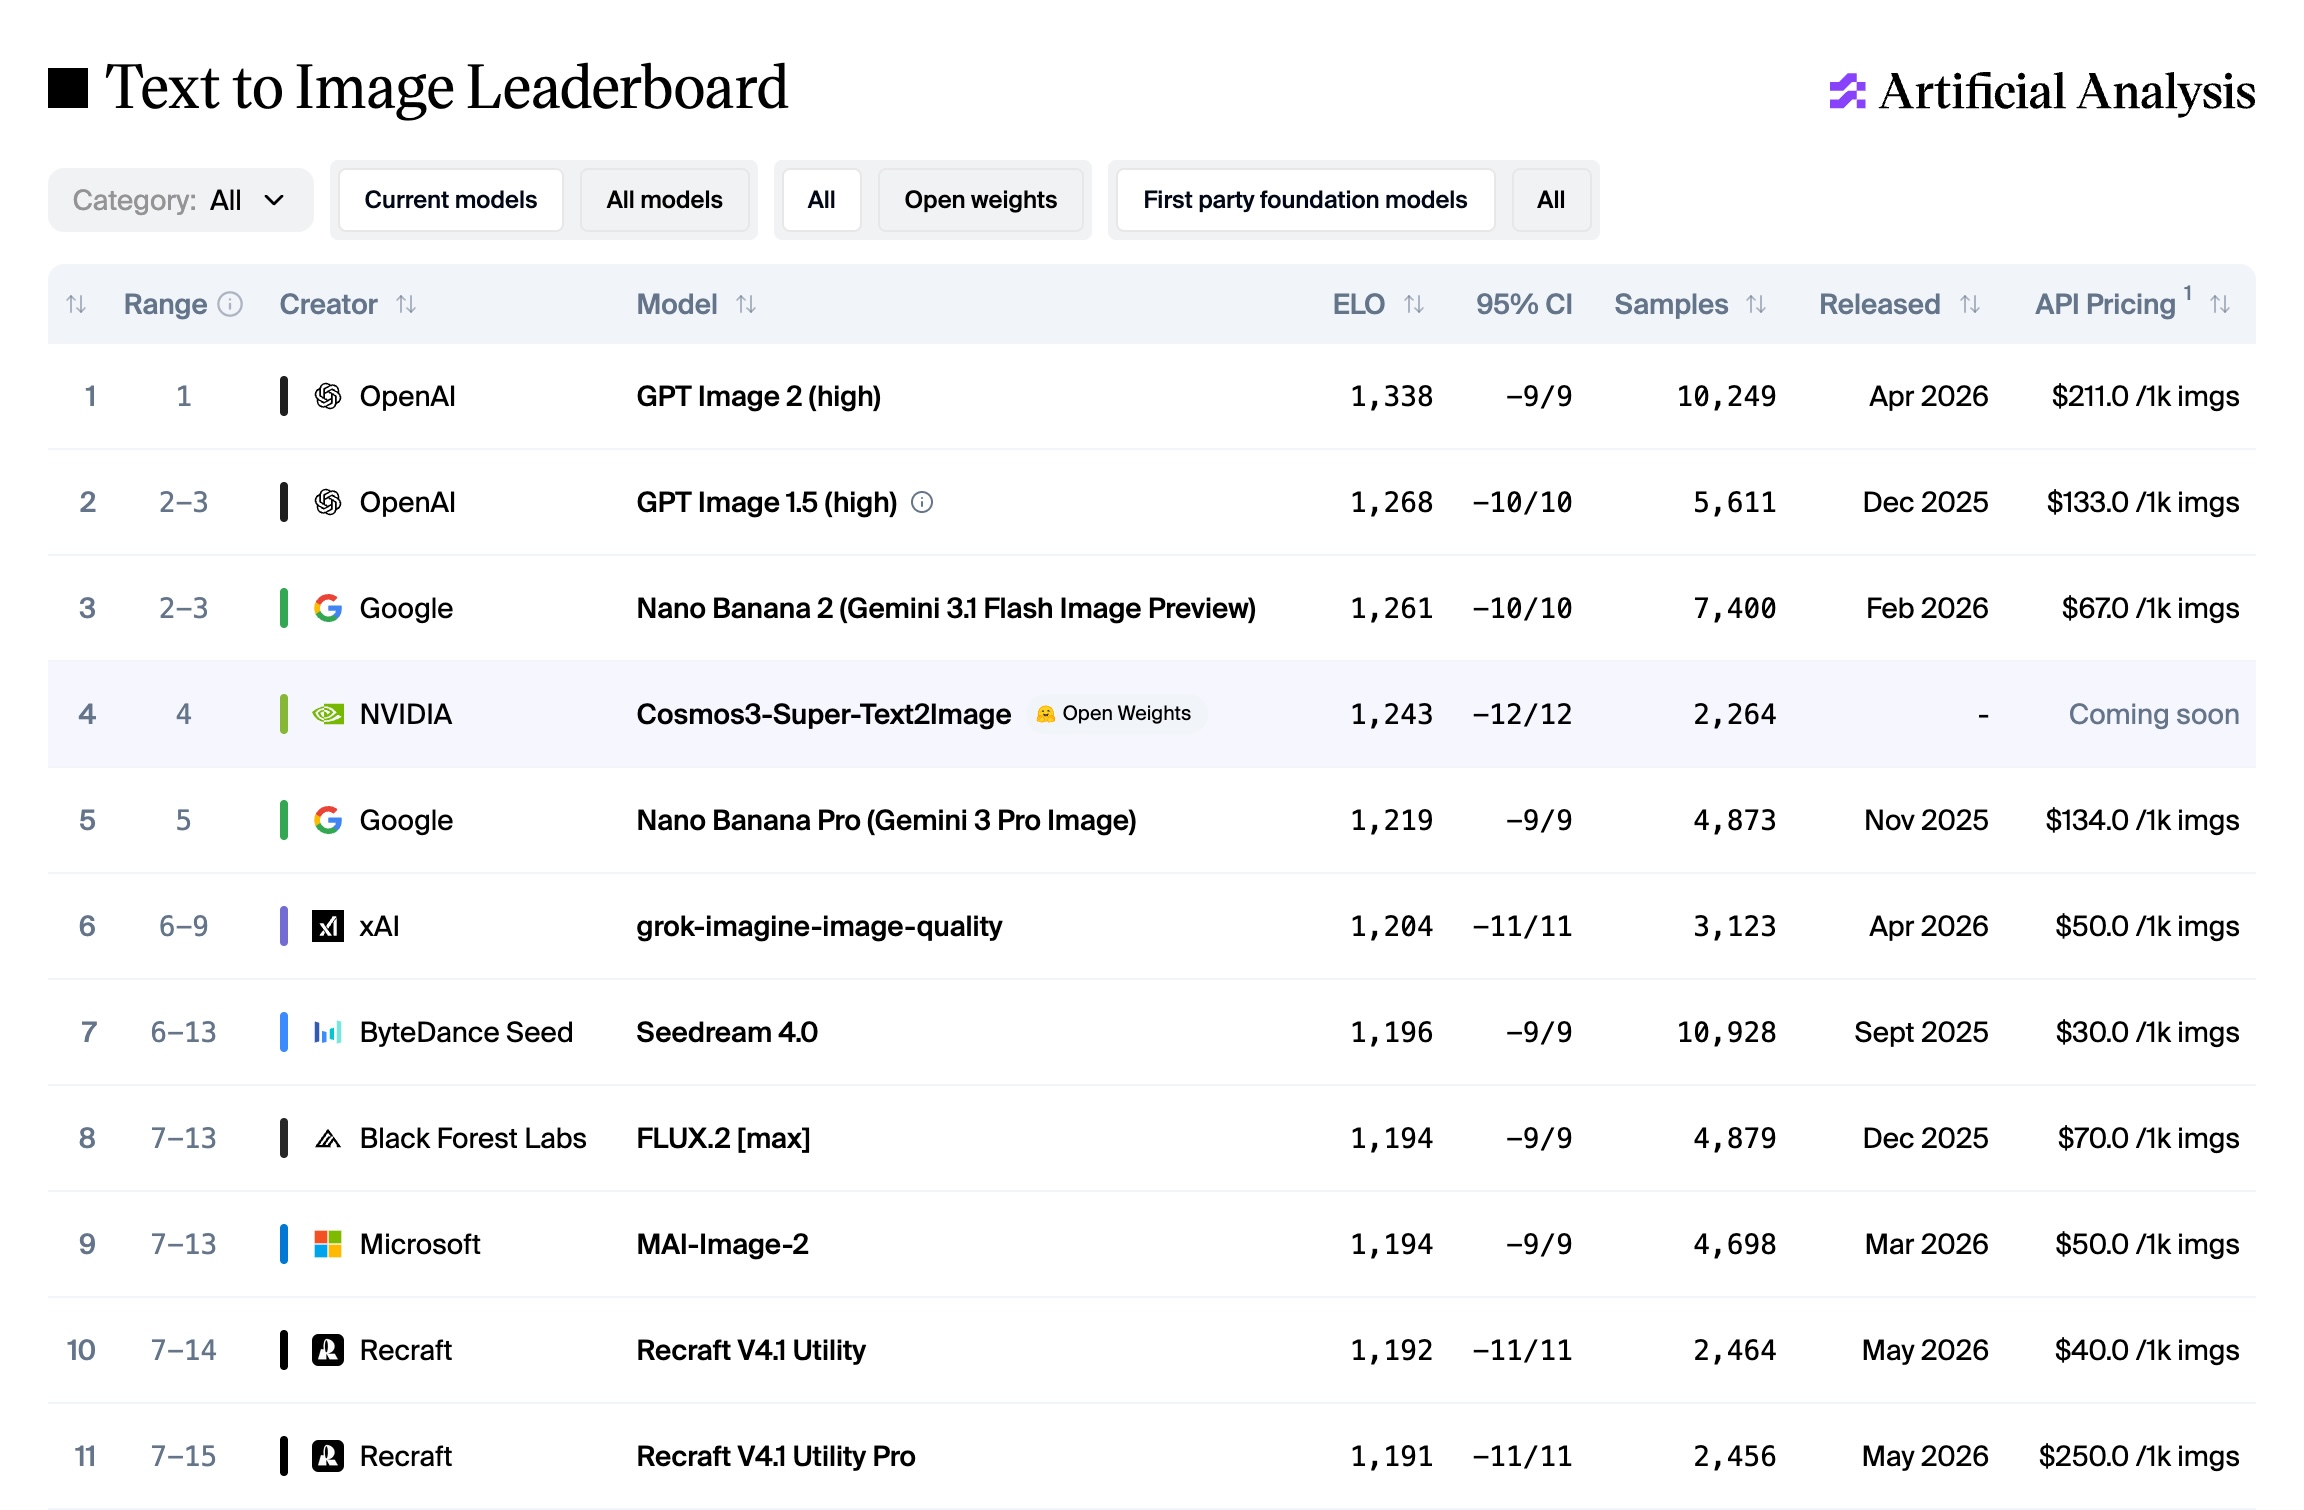
\includegraphics[width=\linewidth]{figures/results/sft_t2i/2026-05-28-Cosmos3-Super-Text2Image-Leaderboard}
    \caption{\textbf{Cosmos3-Super-Text2Image is the \#1 open-weight model on crowdsourced arena rankings.} \textbf{Cosmos3-Super-Text2Image} ranked \#1 among open-weight models (\#4 including proprietary models) on the Artificial Analysis Text to Image Leaderboard (Date: 2026-05-28).}
    \label{fig:sft_t2i_aa_leaderboard}
    \vspace{-0.5\baselineskip}
\end{figure}

\paragraph{Artificial Analysis Text-to-Image Leaderboard.} To evaluate Cosmos 3 under real-world scenarios, we submitted our specialized T2I model, Cosmos3-Super-Text2Image, alongside an agentic harness, to the Artificial Analysis Text-to-Image leaderboard for crowdsourced public voting. The model ranked \#1 among all open-weight models and \#4 among all models (open $+$ closed). For more details on the submission, please see Appendix ~\ref{appendix:t2i_agentic_upsampling}.
